\section{Eight priced corrections}
\label{app:defects} Each of the following was found by re-reading committed artifacts, not by
running new experiments. Items 1--5 were harness defects --- the measurement
itself was contaminated. Items 6--8 were claims withdrawn after correction
--- the measurement was sound, but the claim drawn from it was not. Five of
the eight biased against the autoregressive arm. \begin{enumerate}
\item \textbf{Decoding configuration.} Qwen's checkpoint sets
\texttt{repetition\_penalty}\,$=$\,1.1, which suppresses span-copying and
empties the \texttt{host} field. Correcting to 1.0 moved AR 9-field F1 from
\defectOneFBefore{} to \defectOneFAfter. \emph{Against AR.} \item \textbf{Serving parity.} The AR model ran a naive HuggingFace generate
loop while the diffusion model ran on vLLM with continuous batching. Moving
AR to vLLM moved its p50 from \defectTwoBefore{} to \defectTwoAfter\,ms
(\defectTwoRatio$\times$), reversing the headline speed claim.
\emph{Against AR.} \item \textbf{Parser policy.} At $L{=}512$, \rambleRate\% of AR outputs
contained multiple JSON objects. The old parser took the last (most-drifted)
copy; first-object-wins moved AR F1 from \defectThreeBefore{} to
\defectThreeAfter. \emph{Against AR.} \item \textbf{Metric defaults.} The completeness metric treated falsy values
(\texttt{""}, \texttt{0.0}, \texttt{False}) as missing keys. The AR model
emits falsy defaults on early stop; DiffusionGemma always fills every field.
Distinguishing absent from present-but-falsy moved AR completeness from
\defectFourBefore\% to \defectFourAfter\%. \emph{Against AR.} \item \textbf{Provenance.} A CLI default wrote an AR model name into three DG
result files. Biases no comparison but made audit impossible until correction
sidecars were written. \emph{Neutral.} \item \textbf{Classical-parser baseline.} An earlier draft claimed a classical
parser matched LLM extraction at Field-F1 of $0.68$ against $0.85$. What was
recorded as a near-match was self-grading: our ``Drain'' was a regex fallback
rather than the reference implementation, and the gold generator was the same
code. The claim is withdrawn. \emph{Neutral} (inflated a third baseline, not
either architecture). Found by re-reading the gold-generation script. \item \textbf{Contaminated semantic gold.} An earlier draft claimed structural
and semantic fields separate cleanly, on a 12-field macro where AR led DG by
\twelveGap\ F1. The semantic gold labels were placeholder output of the same
parser, one a constant across 2{,}000 events. On the decontaminated 9-field
macro the two differ by \qualityGap. The contamination inflated the arm that
fills fields with plausible text (AR) and penalised the arm that leaves them
empty (DG). \emph{Against DG.} Found by re-reading the gold labels. \item \textbf{Queueing model.} An earlier draft claimed an M/D/1 queue
predicts diffusion latency under load. The match was to the measured
saturation knee under Poisson arrivals; under bursty (MMPP) arrivals, which is
what log streams actually produce, the model stops being predictive. The claim
is withdrawn. \emph{Against AR} (overstated how well DG's load behaviour is
modelled).
\end{enumerate} The clustering on one arm is not a coincidence: a comparison harness written by
someone hoping the new architecture wins fails asymmetrically, because the
arm the experimenter is not rooting for inherits the checkpoint defaults, the
naive serving path, and the mature production infrastructure.

\begin{figure}[t]
\centering
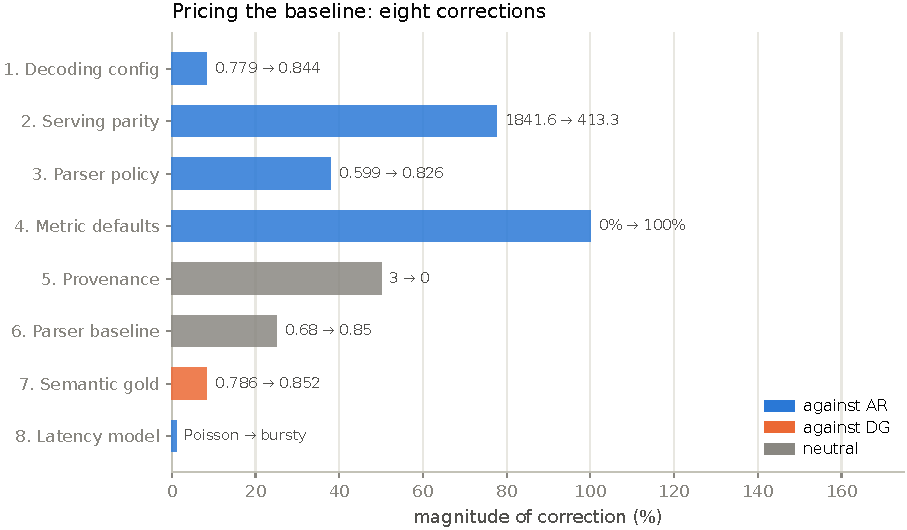
\includegraphics[width=\linewidth]{figures/fig8_defects.pdf}
\caption{Eight priced errors in our own comparison harness, each found by
re-reading committed artifacts (BGL, $n{=}300$ per cell, $K{=}8$). Five
of eight biased against the autoregressive arm.}
\label{fig:defects}
\end{figure}
